\documentclass[a4paper,12pt,french]{article}

\usepackage{../../../Style}

\geometry{top=10mm,bottom=10mm}

\renewcommand\tabularxcolumn[1]{m{#1}}

\setlist[itemize]{align=parleft,left=5pt..20pt}
\setlist[enumerate]{align=parleft,left=5pt..20pt}

\renewcommand{\emph}[2][black]{\textcolor{#1}{\textbf{#2}}} % Bof, a ne pas refaire

\pagestyle{empty}

% Début du document
%%%%%%%%%%%%%%%%%%%
\begin{document}

\newcommand{\contenu}
{
\begin{propr} 
Dans un repère, la représentation graphique d'une fonction affine est une \emph{droite} qui coupe l'axe des ordonnées.
\end{propr}

\begin{enonce}{Vocabulaire}
Dans un repère, soit $d$ la droite représentant une fonction affine $f:x \mapsto ax+b$. On dit que:
\begin{itemize}
\item $a$ est le \emph{coefficient directeur} de $d$.
\item $b$ est \emph{l'ordonnée à l'origine} de $d$.
\item $y=ax+b$ est l'équation réduite de $d$.
\end{itemize}
\end{enonce}

\begin{ex} \
\begin{centrer}
\begin{tikzpicture}
\begin{axis}[
styleglobal,
width=0.9*\linewidth,
xmin=-3, xmax=9,
ymin=-2, ymax=3,
xtick distance=1,
ytick distance=1,
]
\addplot[styleplot,domain=(-9:9)]{2*x-1};
\addplot[color=red,styleplot,densely dashed,domain=(-9:9)]{-0.5*x+2};
\legend{$f:x \mapsto 2x-1$,$g:x \mapsto -0.5x+2$};
\end{axis}
\end{tikzpicture}
\end{centrer}
\end{ex}
}

\newcommand{\contenua}{

\begin{methode} \

\begin{centrer}
\begin{tikzpicture}
\begin{axis}[
styleglobal,
width=0.9*\linewidth,
xmin=-2, xmax=11,
ymin=-1, ymax=4,
xtick distance=1,
ytick distance=1,
minor x tick num=0,
minor y tick num=0,
]
\addplot[styleplot,domain=(-2:11)]{2*x-1} node[pos=0.33,right] {$d_1$};
\draw[->,>=latex,thick] (1,1) -- (2,1) node[midway,below] {$1$};
\draw[->,>=latex,thick] (2,1) -- (2,3) node[midway,right] {$2$};
\addplot[styleplot,densely dashed,color=blue,domain=(-2:11)]{-1/3*x+3} node[pos=0.8, above right] {$d_2$};
\draw[->,>=latex,thick,color=blue] (3,2) -- (6,2) node[midway,above] {$3$};
\draw[->,>=latex,thick,color=blue] (6,2) -- (6,1) node[midway,right] {$-1$};
\end{axis}
\end{tikzpicture}
\end{centrer}

\begin{itemize}
\item Pour $d_1$: Lorsque j'avance d'un carreau vers la droite, je monte de deux carreaux. Le coefficient directeur de $d_1$ est donc égal à $\frac 2 1=2$. L'ordonnée à l'origine de $d_1$ est $-1$. Alors l'équation réduite de $d_1$ est $y=2x-1$.
\item Pour $d_2$: Lorsque j'avance de trois carreaux vers la droite, je descend d'un carreau. Le coefficient directeur de $d_2$ est donc égal à $\frac {-1} 3$. L'ordonnée à l'origine de $d_1$ est $3$. Alors l'équation réduite de $d_1$ est $y=- \frac 1 3 x+3$.
\end{itemize}
Plus généralement, on a $a=\frac{ \text{déplacement vertical} } {\text{déplacement horizontal}}$.
\end{methode}
}


\newcommand{\contenub}{
\compo[0.5]
{
\begin{centrer}
Si $a>0$:

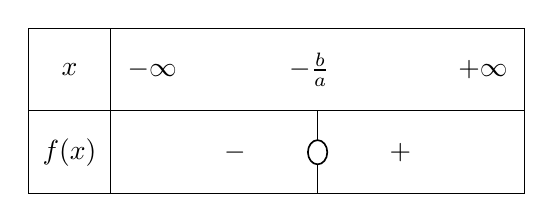
\begin{tikzpicture}[scale=0.875]
% Styles 
\tikzstyle{cadre}=[thin]
\tikzstyle{fleche}=[->,>=latex,thin]
\tikzstyle{nondefini}=[lightgray]
% Dimensions Modifiables
\def\Lrg{1.2}
\def\HtX{1.2}
\def\HtY{0.5}
% Dimensions Calculées
\def\lignex{-0.5*\HtX}
\def\lignef{-1.5*\HtX}
\def\separateur{-0.5*\Lrg}
% Largeur du tableau
\def\gauche{-1.5*\Lrg}
\def\droite{4.5*\Lrg}
% Hauteur du tableau
\def\haut{0.5*\HtX}
\def\bas{-2.5*\HtX-2*\HtY}
% Ligne de l'abscisse : x
\node at (-1*\Lrg,0) {$x$};
\node at (0*\Lrg,0) {$- \infty$};
\node at (1.9*\Lrg,0) {$- \frac b a$};
\node at (4*\Lrg,0) {$+ \infty$};
% Ligne de la dérivée : f'(x)
\node at (-1*\Lrg,-1*\HtX) {$f(x)$};
\node at (1*\Lrg,-1*\HtX) {$-$};
\node at (3*\Lrg,-1*\HtX) {$+$};
\draw[cadre] (2*\Lrg,-0.5*\HtX) -- (2*\Lrg,-1.5*\HtX) node[pos=0.5,line width=0.6pt,draw=black,circle,minimum size=7pt,fill=white,inner sep=2pt,yscale=1.25] {};
% Ligne de la fonction : f(x)
% Encadrement
\draw[cadre] (\separateur,\haut) -- (\separateur, \lignef);
\draw[cadre] (\gauche,\haut) rectangle  (\droite, \lignef);
\draw[cadre] (\gauche,\lignex) -- (\droite,\lignex);
\end{tikzpicture}
\end{centrer}
}
{
\begin{centrer}
Si $a<0$:

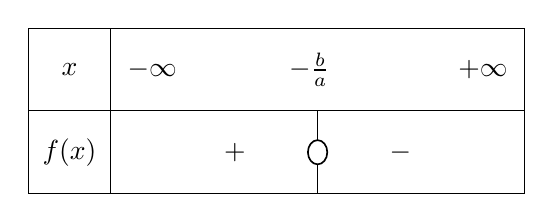
\begin{tikzpicture}[scale=0.875]
% Styles 
\tikzstyle{cadre}=[thin]
\tikzstyle{fleche}=[->,>=latex,thin]
\tikzstyle{nondefini}=[lightgray]
% Dimensions Modifiables
\def\Lrg{1.2}
\def\HtX{1.2}
\def\HtY{0.5}
% Dimensions Calculées
\def\lignex{-0.5*\HtX}
\def\lignef{-1.5*\HtX}
\def\separateur{-0.5*\Lrg}
% Largeur du tableau
\def\gauche{-1.5*\Lrg}
\def\droite{4.5*\Lrg}
% Hauteur du tableau
\def\haut{0.5*\HtX}
\def\bas{-2.5*\HtX-2*\HtY}
% Ligne de l'abscisse : x
\node at (-1*\Lrg,0) {$x$};
\node at (0*\Lrg,0) {$- \infty$};
\node at (1.9*\Lrg,0) {$- \frac b a$};
\node at (4*\Lrg,0) {$+ \infty$};
% Ligne de la dérivée : f'(x)
\node at (-1*\Lrg,-1*\HtX) {$f(x)$};
\node at (1*\Lrg,-1*\HtX) {$+$};
\node at (3*\Lrg,-1*\HtX) {$-$};
\draw[cadre] (2*\Lrg,-0.5*\HtX) -- (2*\Lrg,-1.5*\HtX) node[pos=0.5,line width=0.6pt,draw=black,circle,minimum size=7pt,fill=white,inner sep=2pt,yscale=1.25] {};
% Ligne de la fonction : f(x)
% Encadrement
\draw[cadre] (\separateur,\haut) -- (\separateur, \lignef);
\draw[cadre] (\gauche,\haut) rectangle  (\droite, \lignef);
\draw[cadre] (\gauche,\lignex) -- (\droite,\lignex);
\end{tikzpicture}
\end{centrer}
}}

\contenu

\vfill

\contenu

\newpage

\contenua

\vfill

\contenua

\newpage

\contenub

\vfill

\contenub

\vfill

\contenub

\vfill

\contenub

\vfill

\contenub

\vfill

\contenub

\vfill

\contenub
\end{document}
